\documentclass[a4paper,11pt]{article}
\usepackage[english]{babel}
\usepackage[utf8]{inputenc}
\usepackage[T1]{fontenc}
\usepackage{tikz}
\usepackage{times}
\usetikzlibrary{calc,through,backgrounds,positioning,fit}
\usetikzlibrary{shapes,arrows,shadows}
\usetikzlibrary{mindmap}

\begin{document}

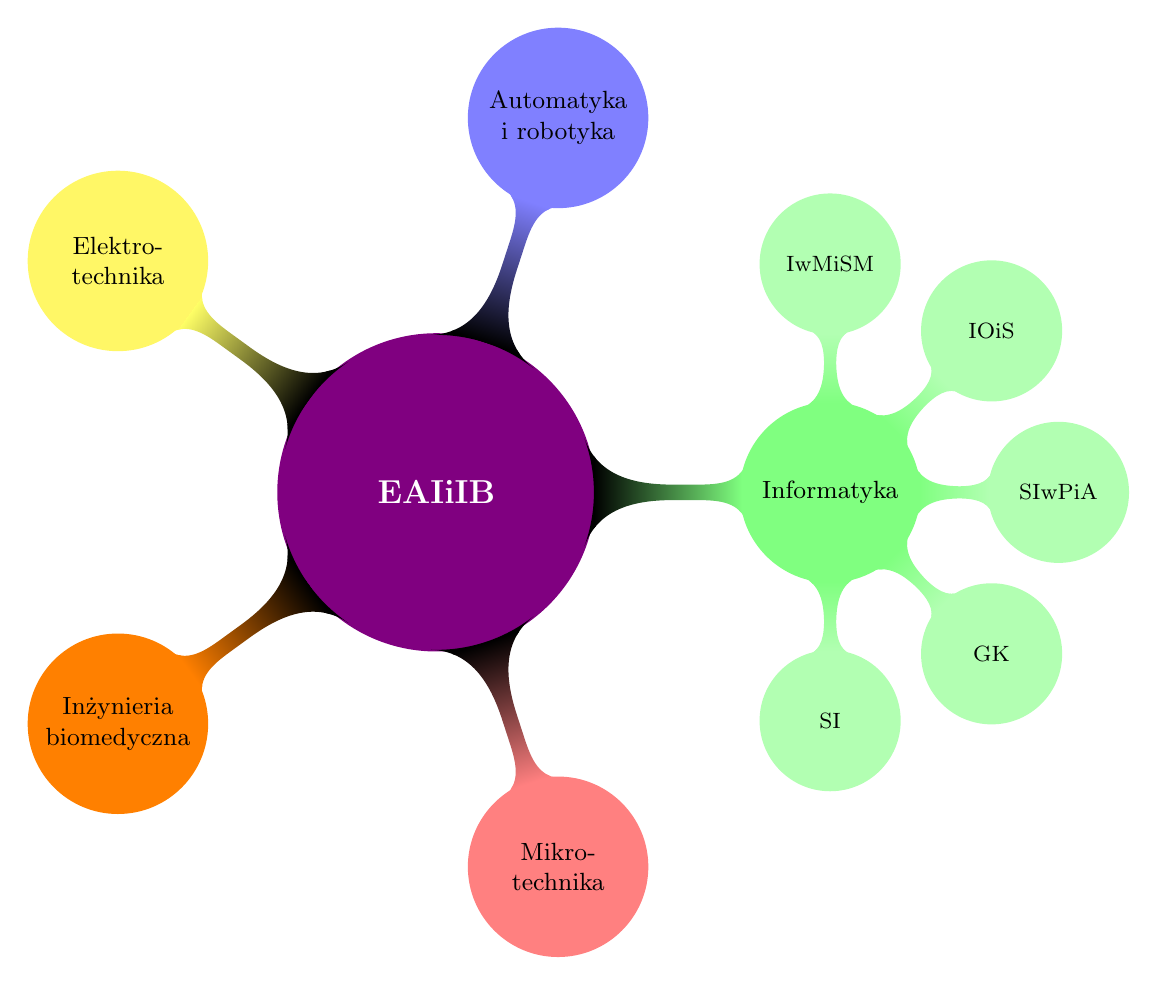
\begin{tikzpicture}[mindmap]
\node [concept,concept color=red!50!blue, text=white] {\bf EAIiIB}
  child[grow=0, concept color=green!50] {node[concept] {Informatyka}
    child[grow=90, concept color=green!30] {node[concept] {IwMiSM}}
    child[grow=45, concept color=green!30] {node[concept] {IOiS}}
    child[grow=0, concept color=green!30] {node[concept] {SIwPiA}}
    child[grow=315, concept color=green!30] {node[concept] {GK}}
    child[grow=270, concept color=green!30] {node[concept] {SI}}
  }
  child[grow=72, concept color=blue!50] {node[concept] {Automatyka i robotyka}}
  child[grow=144, concept color=yellow!60] {node[concept] {Elektro- technika}}
  child[grow=216, concept color=orange!100] {node[concept] {Inżynieria biomedyczna}}
  child[grow=288, concept color=pink!200] {node[concept] {Mikro- technika}}
;
\end{tikzpicture}

\end{document}
